\documentclass[12pt,a4paper]{article}
\usepackage[utf8]{inputenc}
\usepackage[T1]{fontenc}
\usepackage[brazilian]{babel}
\usepackage{amsmath,amssymb}
\usepackage{graphicx}
\usepackage{booktabs}
\usepackage{multirow}
\usepackage{hyperref}
\usepackage{float}
\usepackage{geometry}
\usepackage{algorithm}
\usepackage{algpseudocode}
\usepackage{caption}
\usepackage{subcaption}
\usepackage{xcolor}
\usepackage{enumitem}

\geometry{margin=2.5cm}
\graphicspath{{figures/}}

\title{Análise Topológica da Rede de Transações do Token PEPE \\ sob Choques Geopolíticos e de Mercado}
\author{
  Gabriel Alves de Arruda\textsuperscript{1} \quad Guilherme Brentan de Oliveira\textsuperscript{2} \\[6pt]
  \small Professor Ruben Interian \\
  \small Universidade Estadual de Campinas (UNICAMP) \\
  \small MC859: Projeto em Teoria da Computação, 2026S1
}
\date{}

\begin{document}
\maketitle

% ============================================================================
\section{Introdução}
% ============================================================================

O cenário geopolítico de 2026 tem sido marcado por eventos de instabilidade política com impactos imediatos sobre a economia global. Nesse contexto, os criptoativos representam uma classe particularmente interessante para análise: operam em mercados digitais descentralizados, com negociação contínua e elevada sensibilidade a fatores externos. Além disso, blockchains públicas oferecem transparência transacional: todas as transferências ficam registradas publicamente e podem ser analisadas computacionalmente.

As transações em blockchain podem ser modeladas como um \textbf{grafo direcionado e ponderado}, no qual os vértices representam endereços públicos e as arestas representam transferências de tokens, ponderadas pelo volume transacionado. Essa modelagem permite a aplicação de algoritmos clássicos de análise de grafos para investigar padrões estruturais da rede: concentração de atividade, formação de comunidades, movimentação de grandes agentes e alterações topológicas em períodos de choque.

O objetivo deste projeto é compreender como a rede de transações de um criptoativo se comporta diante de choques externos de naturezas distintas (geopolíticos e de mercado), buscando identificar se diferentes tipos de evento produzem assinaturas topológicas diferenciáveis, e se movimentos abruptos são impulsionados por poucos vértices altamente influentes ou por atividade distribuída. Para maximizar a observabilidade desses efeitos, escolhemos o token PEPE, uma das maiores \textit{memecoins} da rede Ethereum. Por sua natureza predominantemente especulativa, espera-se que o PEPE seja mais sensível a choques externos do que criptoativos consolidados como o Bitcoin.

Selecionamos dois eventos de choque ocorridos em 2026: \textbf{(A)} o sequestro de Nicolás Maduro, em 03/01/2026; \textbf{(B)} o assassinato de Ali Khamenei, em 28/02/2026. Como referência, utilizamos um período de \textit{baseline} correspondente à semana de 16--23/10/2025, com baixa variação de preço.

O principal resultado é que as janelas analisadas produziram perturbações topológicas opostas: enquanto um evento adensou o núcleo da rede, o outro inundou sua periferia. Isso sugere que a natureza do choque, e não apenas sua magnitude, está associada ao tipo de assinatura estrutural observada. Trata-se de um indício, não de uma lei: o estudo compara um evento de cada tipo, e uma das janelas captura um sinal de mercado sobreposto ao geopolítico (Seção~4.3).

% ============================================================================
\section{Coleta de Dados e Instâncias}
% ============================================================================

\subsection{Extração dos dados}

Para cada evento de choque, selecionou-se o intervalo de D$-$3 a D$+$3 (7 dias), de modo a capturar tanto movimentos antecipatórios quanto reações pós-evento, dentro de um horizonte em que a resposta ao choque ainda é observável antes da diluição por outros fatores de mercado. As transações foram extraídas do \texttt{Google BigQuery}, dataset \texttt{crypto\_ethereum.token\_transfers}, filtrando pelo endereço do contrato PEPE (\texttt{0x6982...1933}):

\begin{verbatim}
SELECT from_address, to_address, block_timestamp,
       SAFE_CAST(value AS FLOAT64)/1e18 AS pepe_amount
FROM `bigquery-public-data.crypto_ethereum.token_transfers`
WHERE token_address = '0x6982...1933'
  AND DATE(block_timestamp) BETWEEN 'yyyy-mm-dd' AND 'yyyy-mm-dd'
\end{verbatim}

\subsection{Instâncias geradas}

As transações foram modeladas como multi-dígrafos ponderados, onde cada aresta representa uma transferência individual com atributos: \texttt{edge\_weight} (volume de PEPE), \texttt{timestamp\_str} e \texttt{edge\_id} (hash da transação). Para os algoritmos estáticos, os multi-dígrafos foram convertidos em dígrafos simples, somando os pesos de arestas entre cada par (source, target). Optou-se pela soma para preservar o volume total transacionado, em vez da contagem de transações, já que o volume é a variável economicamente relevante para identificar concentração de capital.

\begin{table}[H]
\centering
\caption{Estatísticas das instâncias geradas.}
\label{tab:instancias}
\begin{tabular}{lrrrrr}
\toprule
Instância & Vértices & Arestas & Grau médio & SCCs & Maior SCC \\
\midrule
Baseline        & 15.311  & 38.760   & 5,06  & 11.859 & 3.315 \\
Maduro          & 22.799  & 111.380  & 9,77  & 16.929 & 5.756 \\
Khamenei        & 18.469  & 42.510   & 4,60  & 16.111 & 2.319 \\
\bottomrule
\end{tabular}
\end{table}

\subsection{Dados de preço}

Complementamos a análise on-chain com dados de preço diário do PEPE/USD obtidos via CoinGecko. O preço do PEPE subiu 73\% durante a janela Maduro (de \$4,14$\times10^{-6}$ para \$7,15$\times10^{-6}$), com o volume de mercado passando de 195M para 1,79B USD no dia do sequestro. Na janela Khamenei, o preço caiu 10,9\%, sem reação perceptível ao assassinato (Figura~\ref{fig:preco}).

\begin{figure}[H]
\centering
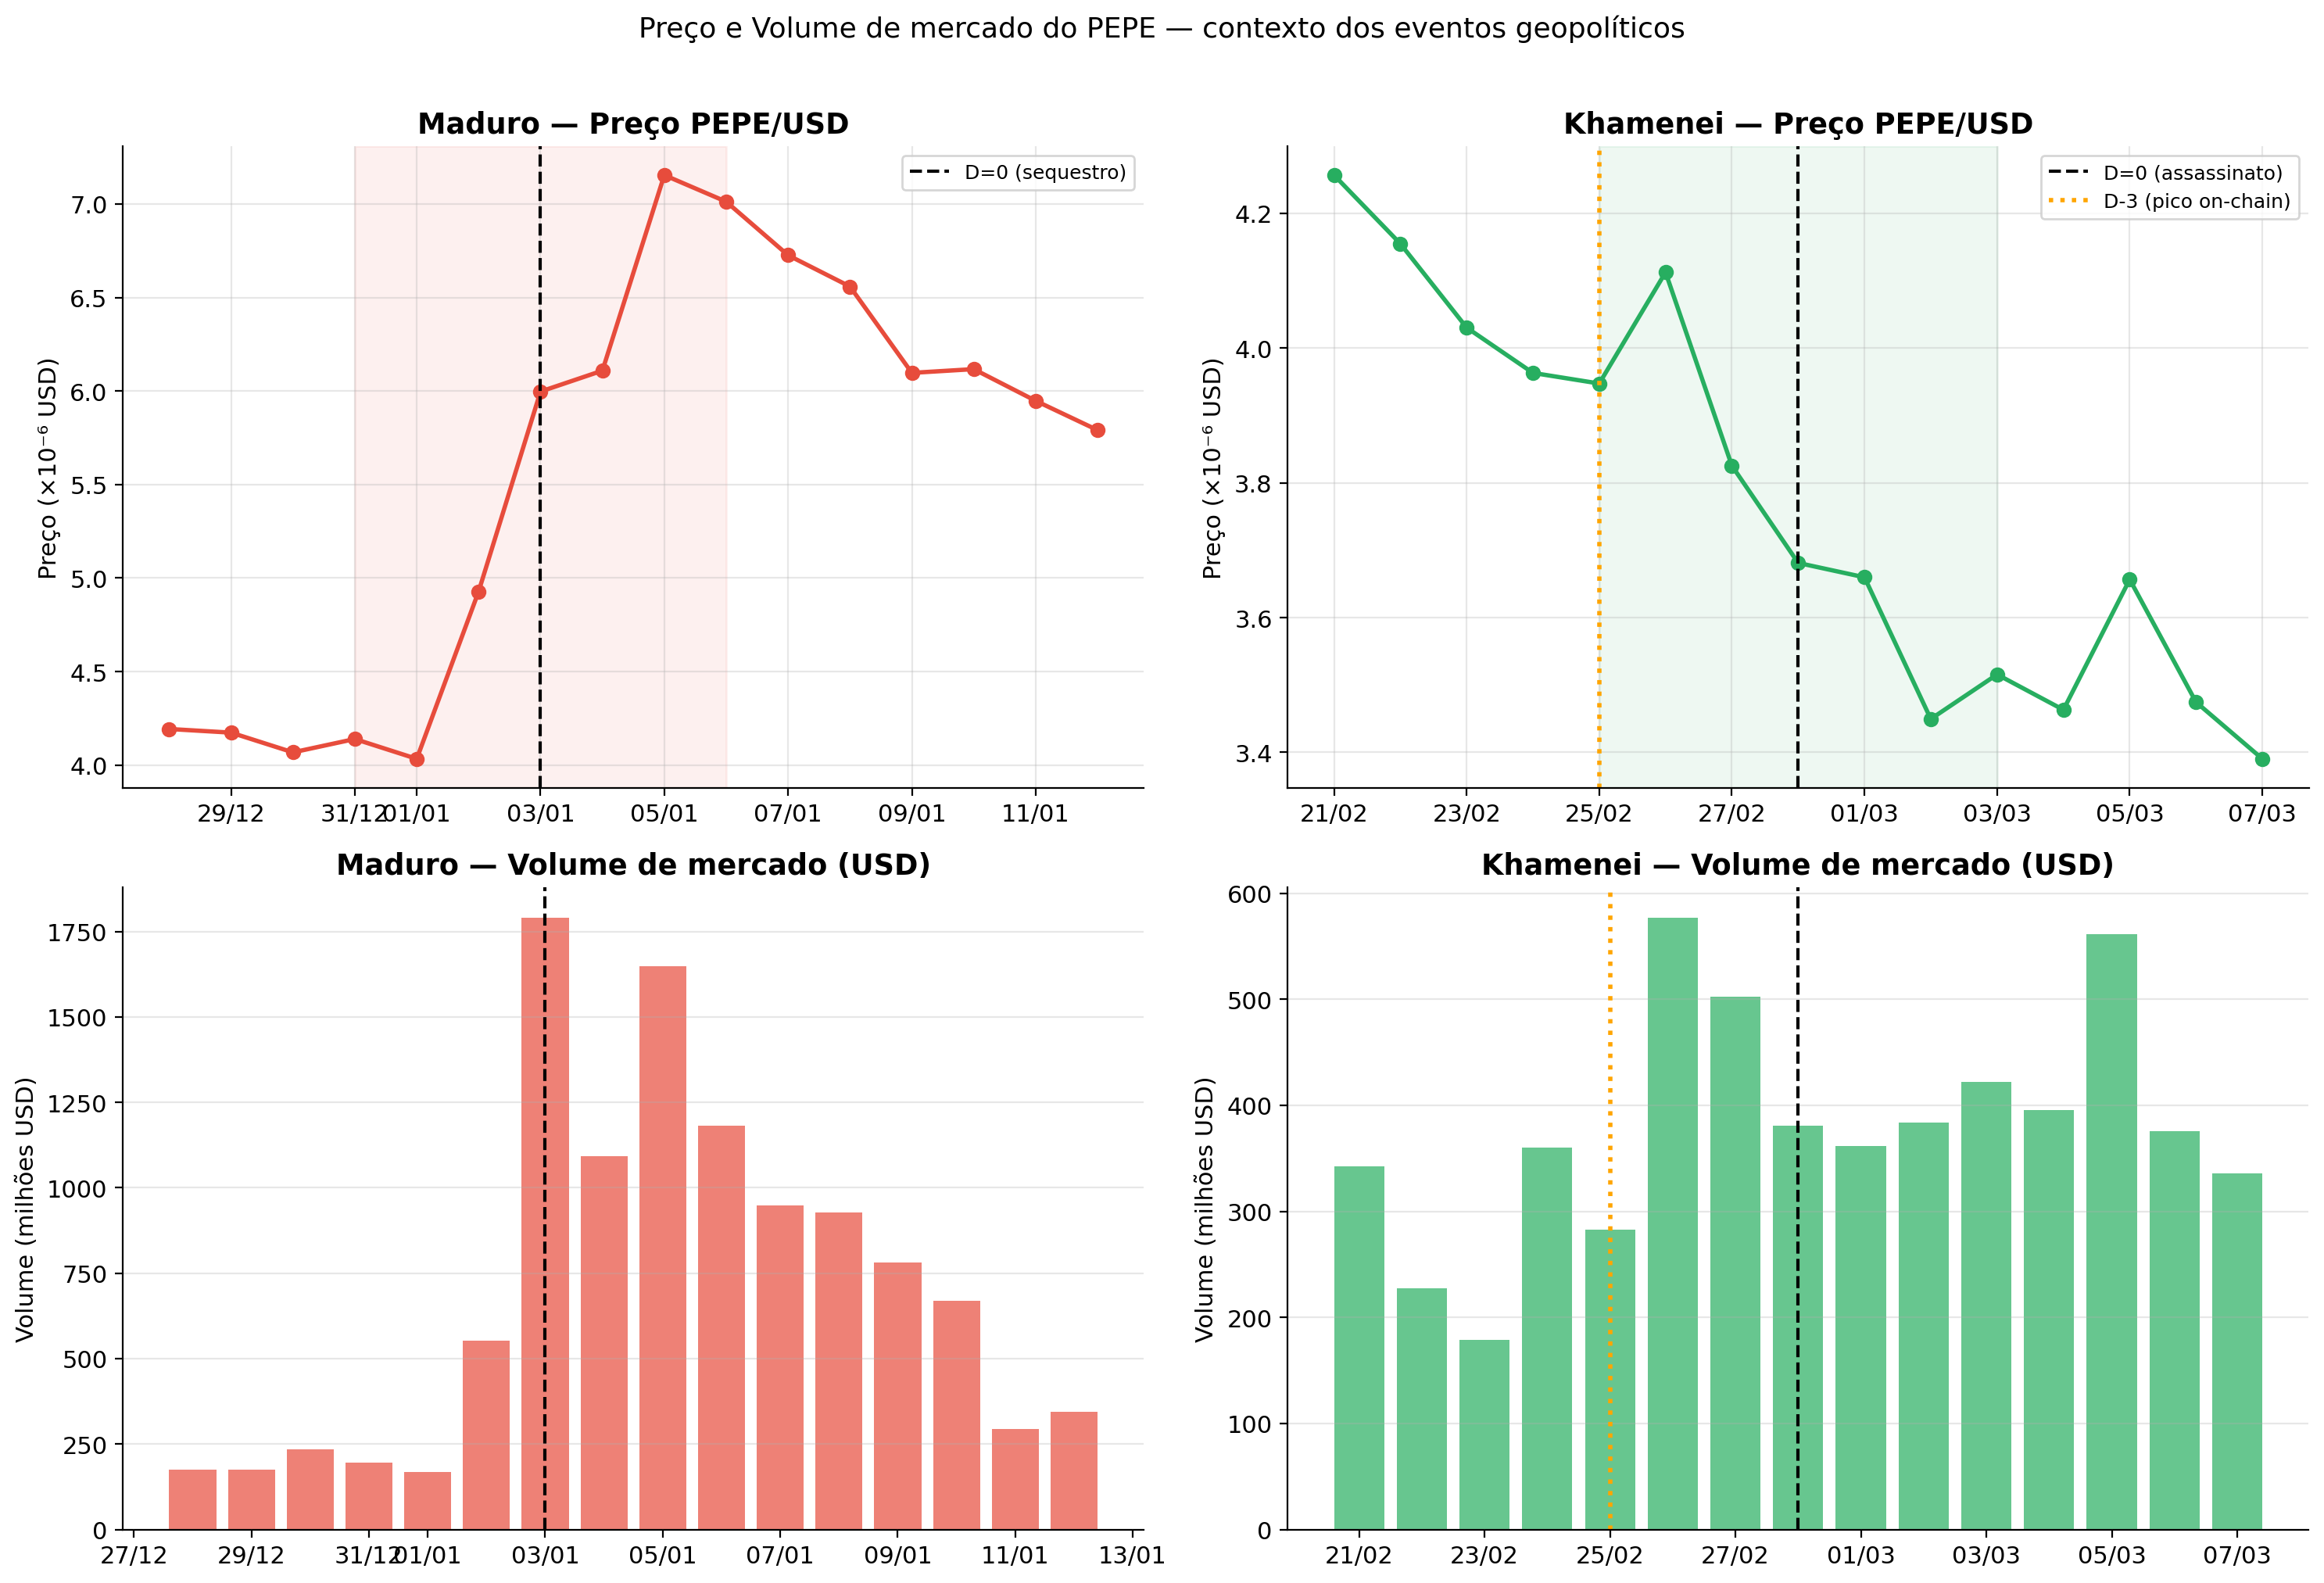
\includegraphics[width=\textwidth]{report_preco_volume.png}
\caption{Preço e volume de mercado diário do PEPE/USD nas janelas dos dois eventos. Na janela Maduro, preço e volume sobem de forma sustentada; na janela Khamenei, o preço declina e o volume de mercado permanece moderado, apesar do pico de atividade on-chain em D$-$3.}
\label{fig:preco}
\end{figure}

% ============================================================================
\section{Algoritmos}
% ============================================================================

Aplicamos oito algoritmos organizados em duas categorias: \textit{extração de conhecimento} (métricas estruturais da rede) e \textit{detecção de padrões} (identificação de anomalias e motifs). A Tabela~\ref{tab:algoritmos} resume a motivação e complexidade de cada um. A proposta inicial previa detecção de comunidades (Louvain); optou-se por k-core, motifs e HITS, mais informativos neste contexto, em que os grafos contêm milhares de nós de grau~1 (singletons da periferia) que tornam a partição em comunidades pouco estável e de baixa interpretabilidade.

\begin{table}[H]
\centering
\caption{Algoritmos aplicados.}
\label{tab:algoritmos}
\small
\begin{tabular}{clll}
\toprule
\# & Algoritmo & Motivação & Complexidade \\
\midrule
\multicolumn{4}{l}{\textit{Extração de Conhecimento}} \\
1 & PageRank + Centralidade & Identificar agentes influentes & $O((n+m) \cdot T)$ \\
2 & Distribuição de Grau    & Verificar regime scale-free    & $O(n \log n)$ \\
3 & Bow-Tie                 & Mapear fluxo direcional        & $O(n+m)$ \\
4 & Análise Temporal         & Localizar anomalias temporais  & $O((n+m) \cdot d)$ \\
\midrule
\multicolumn{4}{l}{\textit{Detecção de Padrões}} \\
5 & K-core                  & Profundidade de integração     & $O(n+m)$ \\
6 & Motifs / Tríades        & Circuitos fechados (arbitragem)& $O(n \cdot \Delta^2)$ \\
7 & Detecção de Anomalia    & Z-scores vs baseline           & $O(k \cdot d)$\textsuperscript{*} \\
8 & HITS                    & Hubs vs Authorities            & $O((n+m) \cdot T)$ \\
\bottomrule
\multicolumn{4}{l}{\footnotesize \textsuperscript{*}$k$ = número de métricas, $d$ = número de dias; custo negligível frente aos algoritmos de grafo.}
\end{tabular}
\end{table}

PageRank~\cite{page1999}, censo de tríades e HITS~\cite{kleinberg1999} foram executados via implementações da biblioteca NetworkX~\cite{networkx} (PageRank com \texttt{weight="edge\_weight"} e \texttt{max\_iter=500}); o ajuste de lei de potência usou a biblioteca \texttt{powerlaw}~\cite{alstott2014}. Apresentamos a seguir o pseudocódigo dos oito algoritmos, na ordem da Tabela~\ref{tab:algoritmos}: os de uso direto de biblioteca na forma adaptada à rede de transações (ponderação por \texttt{edge\_weight}, projeção não-dirigida), e os procedimentos estatísticos (ajuste de lei de potência, agregação temporal) na forma de etapas numeradas. O crédito de implementação e o pseudocódigo coexistem: o segundo documenta a adaptação ao domínio, não a transcrição do método padrão.

\subsection{PageRank Ponderado por Volume}

Adaptamos o PageRank~\cite{page1999} à rede de transações distribuindo o score de cada endereço proporcionalmente ao volume (\texttt{edge\_weight}) de suas arestas de saída, e não uniformemente entre os vizinhos: transferências maiores transmitem mais influência.

\begin{algorithm}[H]
\caption{PageRank Ponderado por Volume}
\begin{algorithmic}[1]
\Require Dígrafo $G=(V,E)$ com pesos $w_{uv}=$ \texttt{edge\_weight}; fator $d=0{,}85$
\Ensure $\text{PR}(v)$ para cada $v \in V$
\ForAll{$v \in V$} $\text{PR}(v) \gets 1/|V|$ \EndFor
\For{$t = 1$ \textbf{até} \texttt{max\_iter}}
  \ForAll{$v \in V$}
    \State $\displaystyle \text{PR}'(v) \gets \frac{1-d}{|V|} + d \!\!\sum_{(u,v)\in E}\!\! \text{PR}(u)\,\frac{w_{uv}}{\sum_{(u,x)\in E} w_{ux}}$
  \EndFor
  \State \textbf{se} $\|\text{PR}'-\text{PR}\|_1 < \varepsilon$ \textbf{então pare}; \quad $\text{PR} \gets \text{PR}'$
\EndFor
\end{algorithmic}
\end{algorithm}

\subsection{Distribuição de Grau}

A verificação do regime de cauda pesada é um procedimento estatístico, não um algoritmo de grafo:

\begin{enumerate}[nosep,leftmargin=*]
\item Extrair a sequência de in-degree (e out-degree) de todos os vértices de $G$.
\item Ajustar uma lei de potência $P(k) \sim k^{-\alpha}$ por máxima verossimilhança~\cite{alstott2014}, estimando o expoente $\alpha$ e o corte inferior $k_{\min}$.
\item Calcular a razão de log-verossimilhança $R$ (e o $p$-valor) entre a lei de potência e uma log-normal; $R \approx 0$ indica que as duas hipóteses são indistinguíveis nos dados.
\end{enumerate}

\subsection{Decomposição Bow-Tie}

A decomposição bow-tie~\cite{broder2000} particiona o grafo em quatro componentes, revelando o fluxo direcional de capital:

\begin{algorithm}[H]
\caption{Decomposição Bow-Tie}
\begin{algorithmic}[1]
\Require Dígrafo $G = (V, E)$
\Ensure Conjuntos SCC, IN, OUT, OTHER
\State $\text{SCCs} \gets$ componentes fortemente conexos de $G$
\State $\text{SCC}_g \gets \arg\max_{S \in \text{SCCs}} |S|$
\State Escolher $s \in \text{SCC}_g$
\State $\text{Forward} \gets \text{BFS}(G, s)$ \Comment{nós alcançáveis a partir de $s$}
\State $\text{Backward} \gets \text{BFS}(G^R, s)$ \Comment{nós que alcançam $s$ no reverso}
\State $\text{IN} \gets \text{Backward} \setminus \text{SCC}_g$
\State $\text{OUT} \gets \text{Forward} \setminus \text{SCC}_g$
\State $\text{OTHER} \gets V \setminus (\text{SCC}_g \cup \text{IN} \cup \text{OUT})$
\end{algorithmic}
\end{algorithm}

\subsection{Agregação Temporal}

A análise temporal é um meta-procedimento que reaplica as métricas dos demais algoritmos a recortes diários do grafo, usando os timestamps das arestas:

\begin{algorithm}[H]
\caption{Agregação Temporal de Métricas}
\begin{algorithmic}[1]
\Require Multi-dígrafo $G$ com timestamps; conjunto de métricas $\mathcal{M}$ (Alg.\ 1--3, 5--6)
\Ensure Série temporal $\{\text{métricas}(d)\}_d$
\ForAll{dia $d$ na janela}
  \State $G_d \gets$ subgrafo de $G$ com arestas cujo timestamp pertence a $d$
  \State Computar cada métrica de $\mathcal{M}$ sobre $G_d$ e registrar em $d$
\EndFor
\end{algorithmic}
\end{algorithm}

\subsection{K-core Decomposition}

O k-core atribui a cada nó $v$ o maior $k$ tal que $v$ pertence ao subgrafo maximal onde todos têm grau $\geq k$~\cite{batagelj2003}. Aplicamos o algoritmo sobre a projeção não-dirigida do grafo para capturar integração bidirecional entre endereços, independentemente da direção da transferência:

\begin{algorithm}[H]
\caption{K-core Decomposition}
\begin{algorithmic}[1]
\Require Grafo não-dirigido $G_u$ (projeção de $G$)
\Ensure $\text{core}(v)$ para cada $v \in V$
\ForAll{$v \in V$} $\text{deg}(v) \gets \text{degree}(v)$ \EndFor
\State $k \gets 0$
\While{existem nós não removidos}
  \State $k \gets k + 1$
  \While{$\exists v : \text{deg}(v) < k$}
    \State $\text{core}(v) \gets k - 1$
    \State Remover $v$; atualizar $\text{deg}$ dos vizinhos
  \EndWhile
\EndWhile
\end{algorithmic}
\end{algorithm}

\subsection{Motifs e Censo de Tríades}

O censo de tríades classifica cada subconjunto conexo de três vértices segundo o padrão de arestas dirigidas presentes, identificando circuitos fechados (tríades 300 e 030C) associados a \textit{trading} cíclico ou arbitragem. A varredura percorre, para cada vértice, os pares de seus vizinhos, o que conduz à complexidade $O(n \cdot \Delta^2)$:

\begin{algorithm}[H]
\caption{Censo de Tríades e Contagem de Triângulos}
\begin{algorithmic}[1]
\Require Dígrafo $G=(V,E)$
\Ensure Contagem por tipo de tríade (030C, 030T, 300, \dots) e nº de triângulos
\State $\text{census}[\,\cdot\,] \gets 0$
\ForAll{$v \in V$}
  \ForAll{par de vizinhos $\{u,w\}$ de $v$, com $u,w \neq v$}
    \State $t \gets$ classificar $(u,v,w)$ pelas arestas dirigidas presentes
    \State $\text{census}[t] \gets \text{census}[t] + 1$
  \EndFor
\EndFor
\State $\text{triângulos} \gets$ contagem na projeção não-dirigida de $G$
\end{algorithmic}
\end{algorithm}

\subsection{Detecção de Anomalia Estatística}

Construímos uma distribuição de referência a partir dos dias do baseline e calculamos z-scores para cada dia de cada evento:

\begin{algorithm}[H]
\caption{Detecção de Anomalia via Z-score}
\begin{algorithmic}[1]
\Require Métricas diárias do baseline $\mathbf{B}$, do evento $\mathbf{E}$
\Ensure $z_m(d)$ e anomaly\_score$(d)$ para cada dia $d$
\ForAll{métrica $m \in \{$nós, SCC\%, OUT/IN, vol$_{\text{IN}\to\text{SCC}}$, Gini, PR$_{\text{top20}}\}$}
  \State $\mu_m \gets \text{média}(\mathbf{B}[m])$; \quad $\sigma_m \gets \text{desvio}(\mathbf{B}[m])$
\EndFor
\ForAll{dia $d$ do evento}
  \ForAll{métrica $m$}
    \State $z_m(d) \gets (\mathbf{E}[m][d] - \mu_m) / \sigma_m$
  \EndFor
  \State anomaly\_score$(d) \gets \sum_m |z_m(d)|$
\EndFor
\end{algorithmic}
\end{algorithm}

\subsection{HITS: Hubs e Authorities}

O algoritmo HITS~\cite{kleinberg1999}, originalmente proposto para grafos de citação na web, pode ser adaptado para redes de transação: um \textit{hub} é um endereço que envia para muitos destinos relevantes (distribuidor), e uma \textit{authority} é um endereço que recebe de muitos remetentes relevantes (acumulador). Utilizamos a implementação não-ponderada do NetworkX, de modo que os scores refletem a \textit{estrutura de conectividade} (quem envia para quem), e não o volume financeiro das arestas:

\begin{algorithm}[H]
\caption{HITS (Kleinberg)}
\begin{algorithmic}[1]
\Require Dígrafo $G = (V, E)$
\Ensure $h(v)$, $a(v)$ para cada $v$
\ForAll{$v \in V$} $h(v) \gets 1$; $a(v) \gets 1$ \EndFor
\Repeat
  \ForAll{$v \in V$} $a(v) \gets \sum_{(u,v) \in E} h(u)$ \EndFor
  \ForAll{$v \in V$} $h(v) \gets \sum_{(v,w) \in E} a(w)$ \EndFor
  \State Normalizar: $\mathbf{a} \gets \mathbf{a}/\|\mathbf{a}\|_2$; \quad $\mathbf{h} \gets \mathbf{h}/\|\mathbf{h}\|_2$
\Until{convergência}
\end{algorithmic}
\end{algorithm}

% ============================================================================
\section{Resultados}
% ============================================================================

\subsection{O baseline: uma rede de cauda pesada}

O grafo baseline apresenta distribuição de in-degree com expoente $\alpha = 1{,}976$ e razão de log-verossimilhança $R \approx 0$ (lei de potência e log-normal são estatisticamente indistinguíveis). Seguindo Clauset et al., com $R \approx 0$ os dados são \textit{consistentes} com um regime de cauda pesada, mas não permitem distinguir estatisticamente lei de potência de log-normal; tratamos ``scale-free'' como hipótese não-rejeitada, e não como fato confirmado. Notavelmente, $\alpha \approx 2{,}0$ é inferior ao expoente $\gamma \approx 3$ previsto pelo modelo de Barabási-Albert~\cite{barabasi1999}, indicando uma cauda mais pesada: para $\alpha \leq 2$, o segundo momento da distribuição de grau diverge, o que implica alta variabilidade e dominância de hubs extremos. A decomposição bow-tie revela estrutura equilibrada (SCC=22\%, IN=30\%, OUT=34\%), com razão OUT/IN $= 1{,}14$ e transitivity de 0,002.

\begin{figure}[H]
\centering
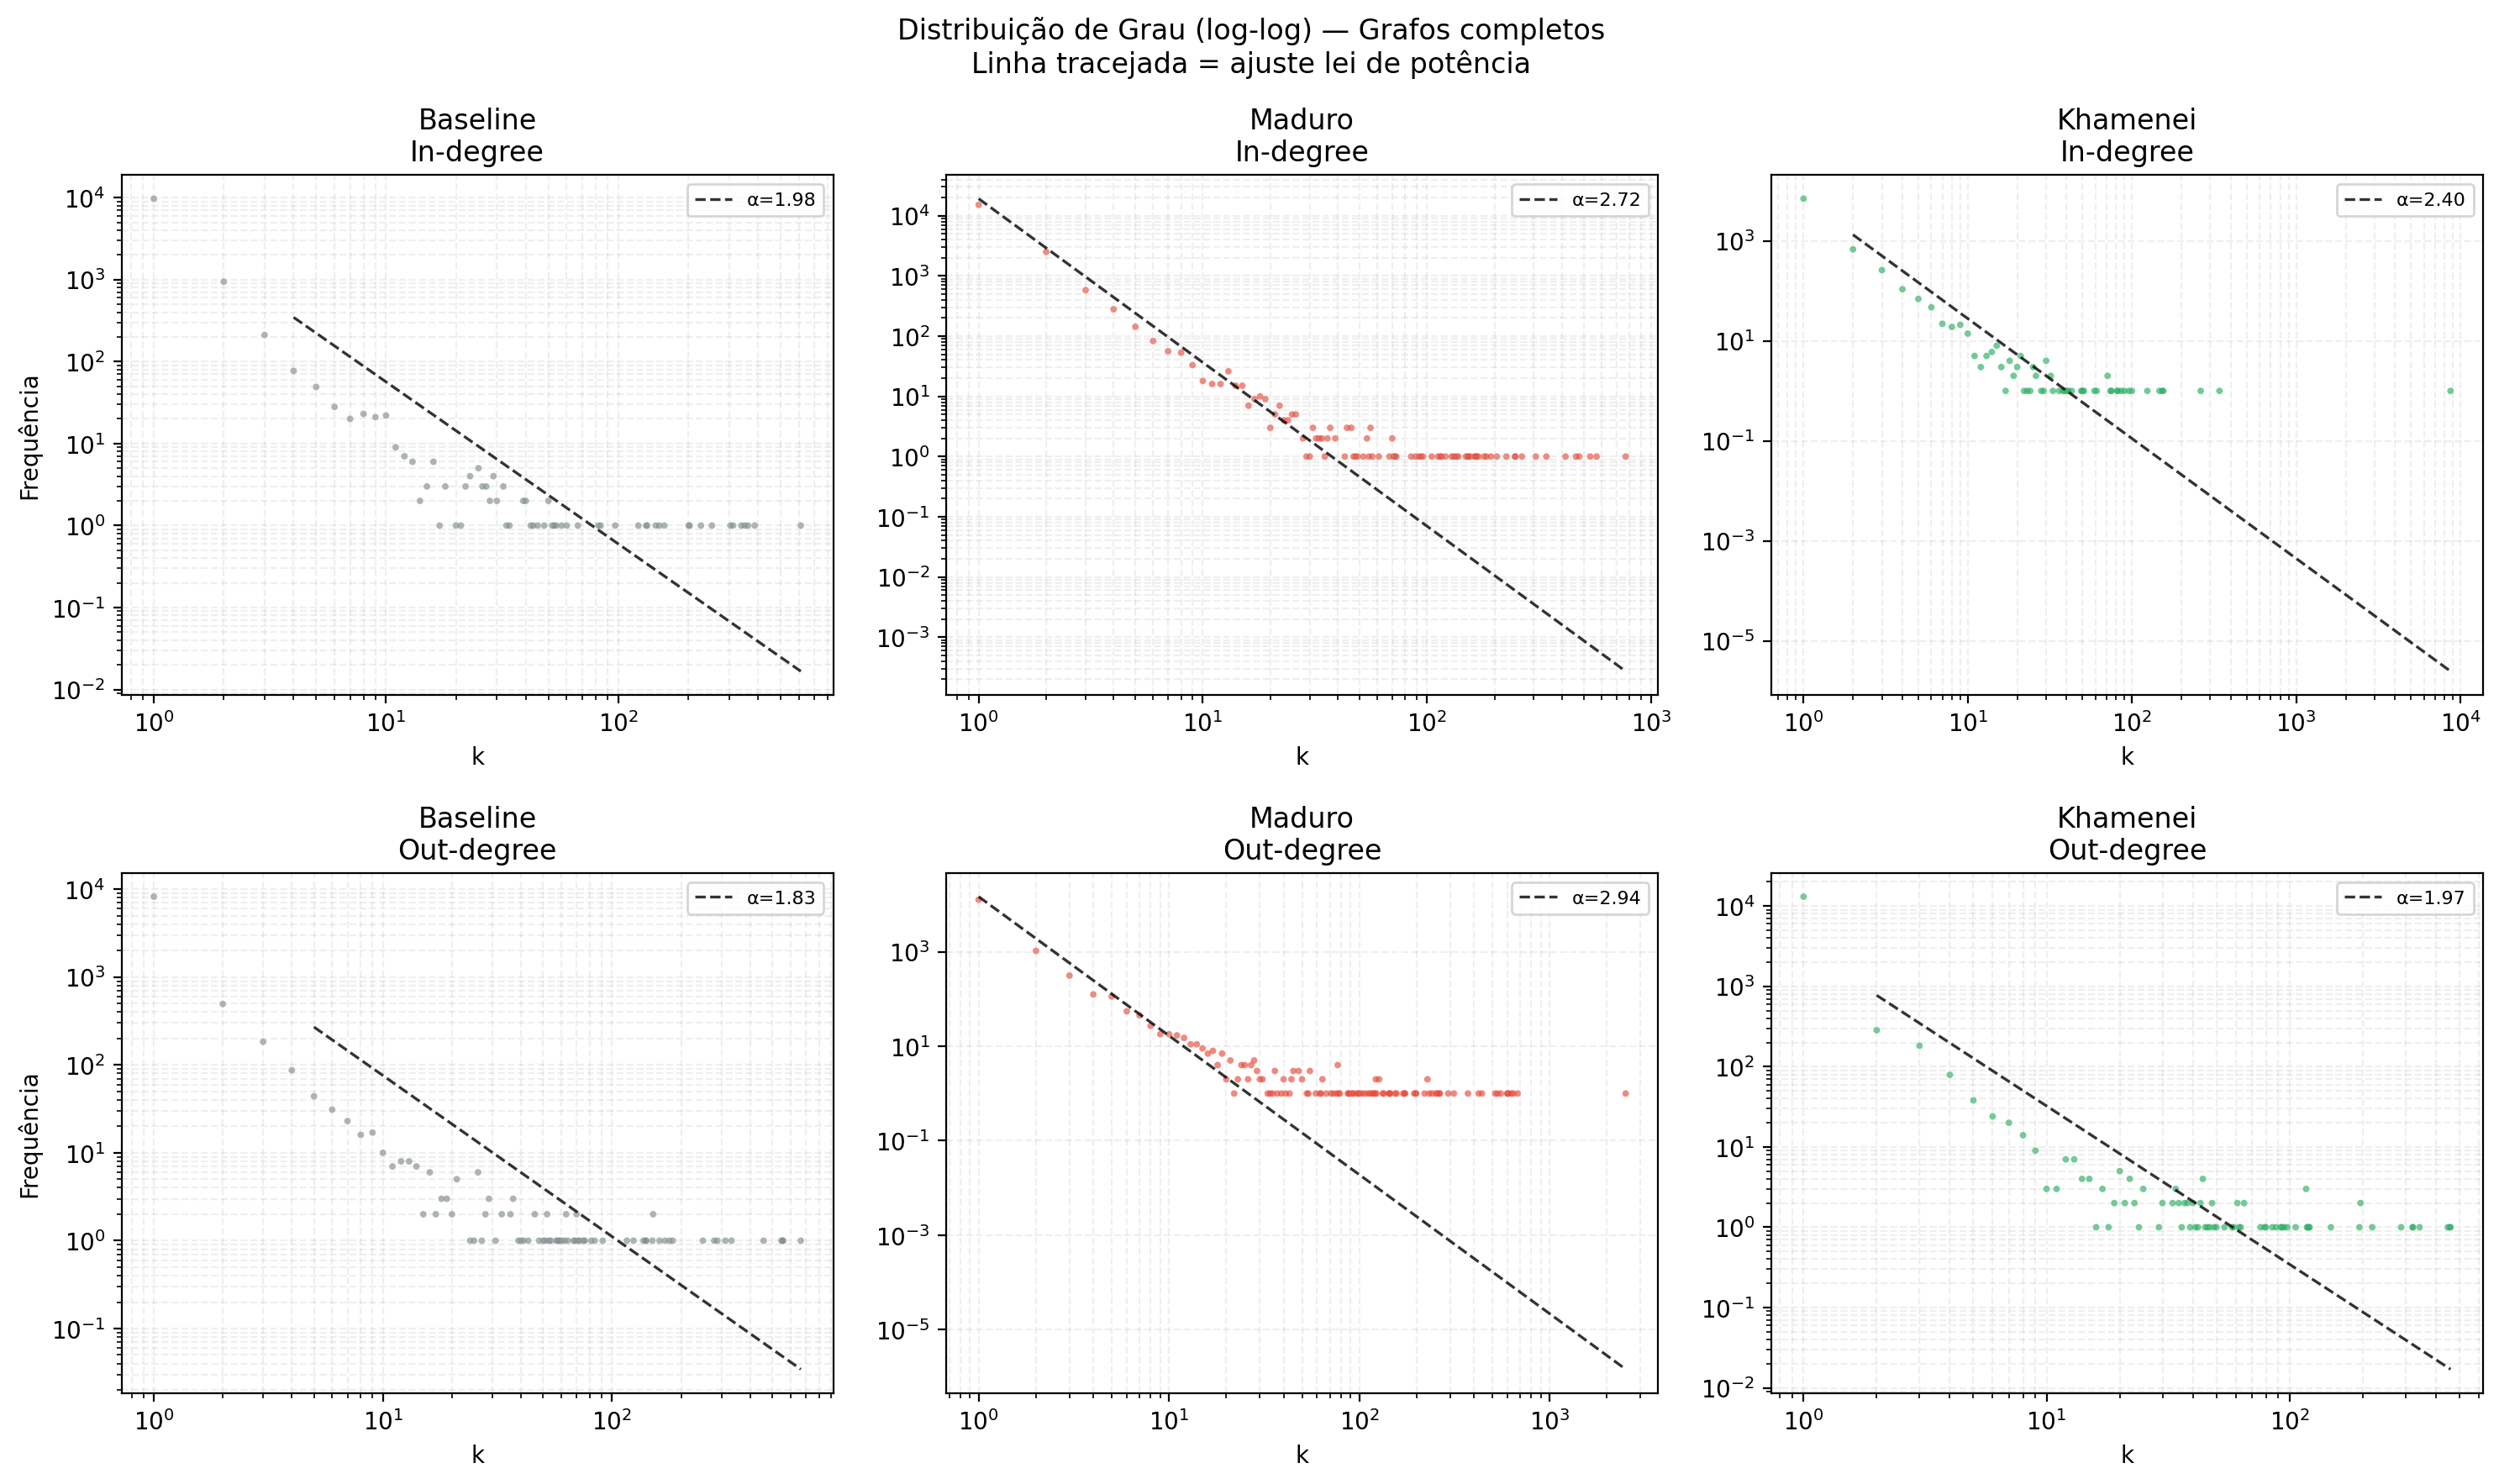
\includegraphics[width=\textwidth]{report_distribuicao_gexf.png}
\caption{Distribuição de in-degree e out-degree (escala log-log) para os três grafos. A linha tracejada indica o ajuste de lei de potência. O baseline ($\alpha \approx 2{,}0$) apresenta distribuição de cauda pesada consistente com regime scale-free, com $\alpha < \gamma_{\text{BA}} \approx 3$.}
\label{fig:grau}
\end{figure}

\subsection{Evento Maduro: adensamento do núcleo}

O sequestro de Maduro coincidiu com uma valorização de 73\% do PEPE e um salto de volume de mercado (1,79B USD no dia do evento, 9,2$\times$ o volume de D$-$3 e cerca de 3,2$\times$ o do dia anterior). As métricas estruturais são consistentes com um adensamento do núcleo da rede:

\begin{table}[H]
\centering
\caption{Comparação de métricas: Baseline vs Maduro vs Khamenei.}
\label{tab:comparacao}
\small
\begin{tabular}{lrrr}
\toprule
Métrica & Baseline & Maduro & Khamenei \\
\midrule
SCC (\% nós) & 21,7\% & \textbf{25,2\%} & 12,6\% \\
IN (\% nós) & 30,0\% & 32,2\% & \textbf{57,6\%} \\
OUT (\% nós) & 34,2\% & 32,8\% & 21,6\% \\
Razão OUT/IN & 1,14 & 1,02 & \textbf{0,38} \\
$k_{\max}$ (K-core) & 8 & \textbf{10} & 8 \\
\% nós $k=1$ & 71,5\% & 51,9\% & \textbf{81,9\%} \\
Triângulos & 1.935 & \textbf{5.601} & 1.605 \\
Tríades 300 & 78 & \textbf{494} & 78 \\
Transitivity & 0,0021 & 0,0018 & \textbf{0,0001} \\
Gini Volume & 0,983 & \textbf{0,992} & 0,989 \\
Top-20 Vol Share & 41,2\% & \textbf{53,1\%} & 46,7\% \\
$\alpha$ in-degree & 1,976 & 2,719 & 2,399 \\
Gini Hub (HITS) & 0,975 & \textbf{1,000} & 0,222 \\
Gini Auth (HITS) & 0,829 & 0,768 & \textbf{1,000} \\
\bottomrule
\end{tabular}
\end{table}

\begin{figure}[H]
\centering
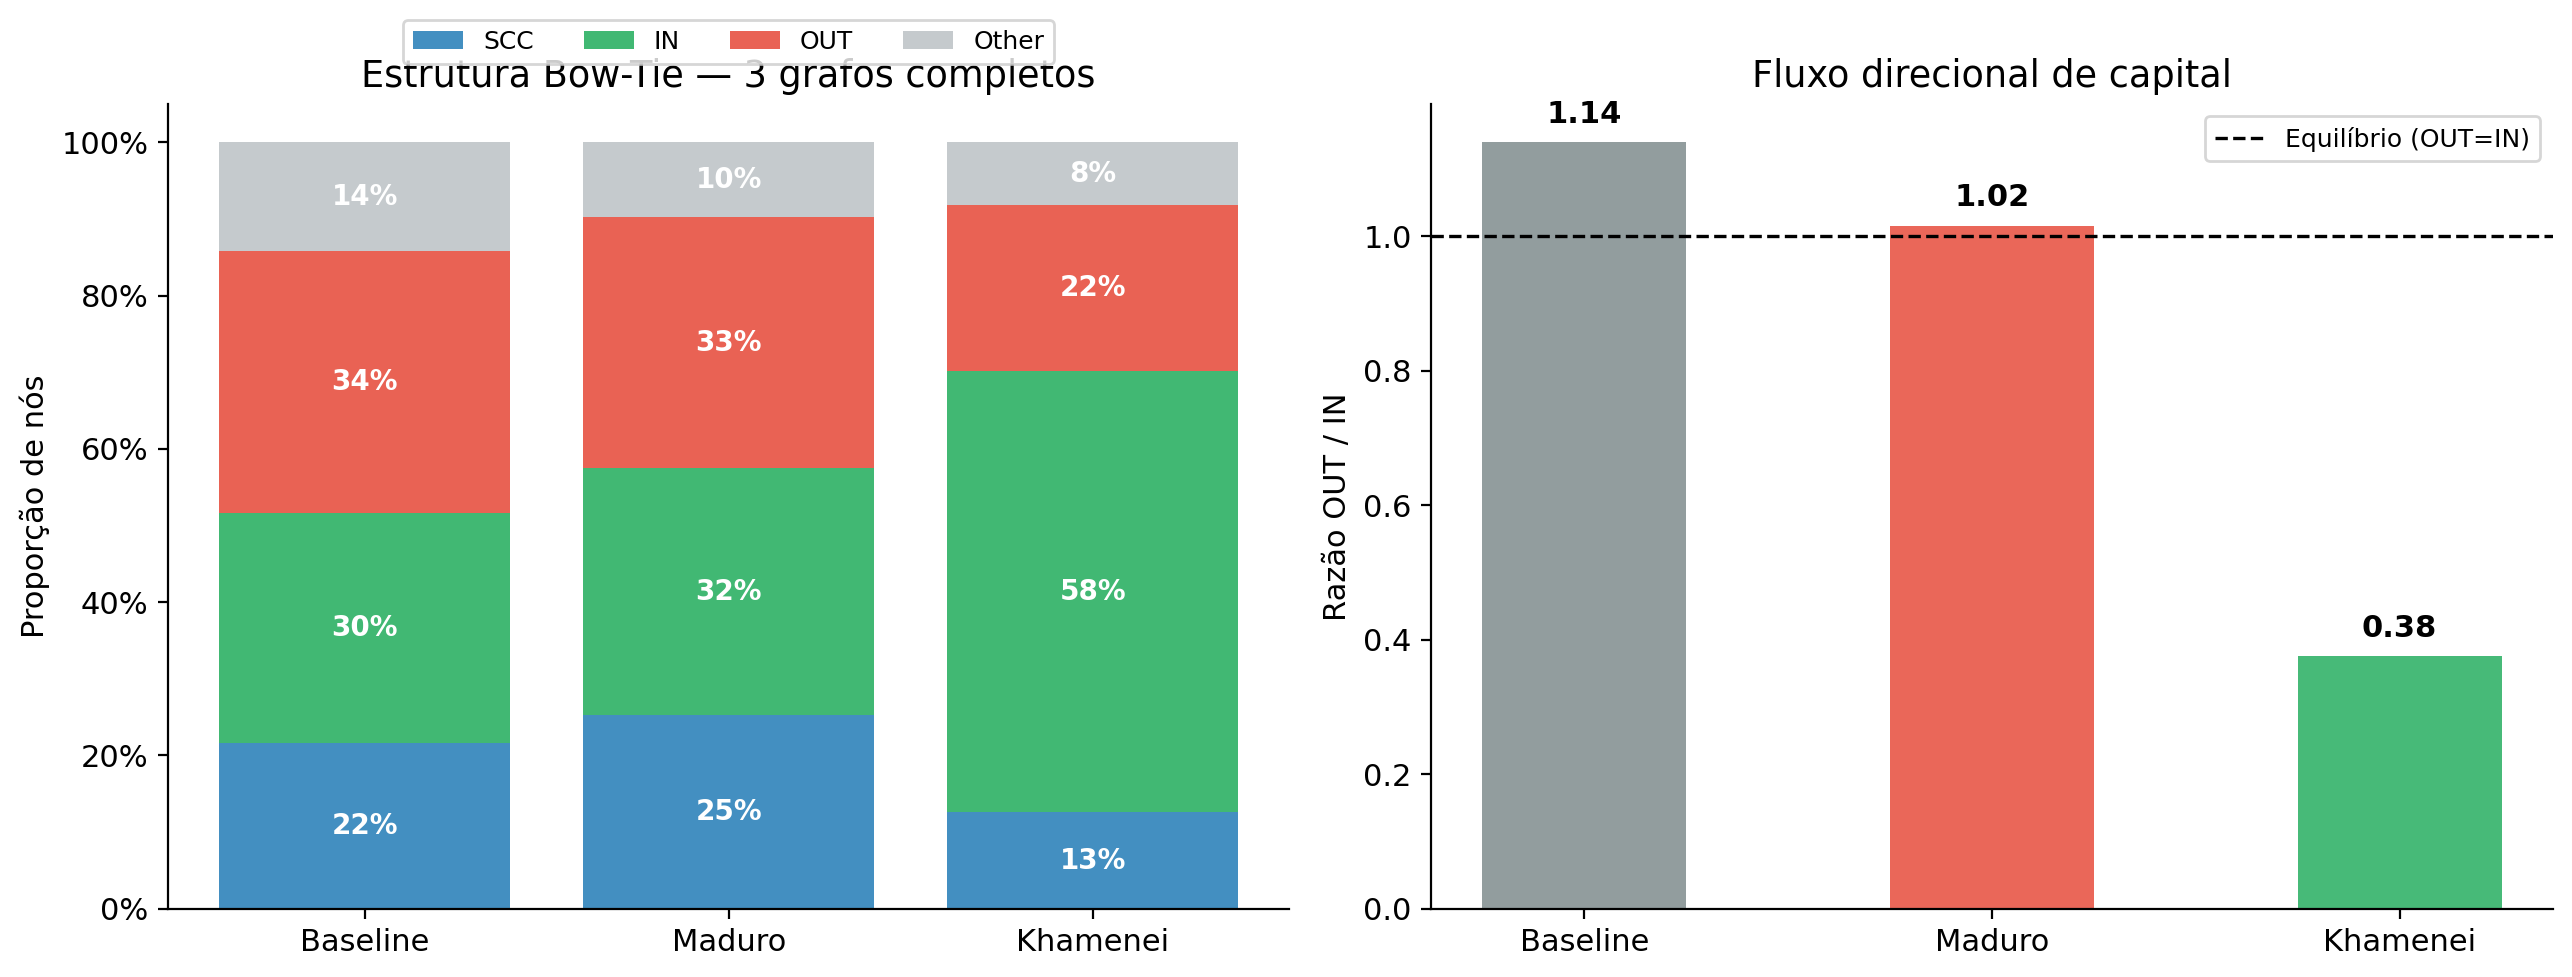
\includegraphics[width=\textwidth]{report_bowtie_gexf.png}
\caption{Decomposição bow-tie e razão OUT/IN para os três grafos. O Khamenei apresenta 57,6\% de nós no componente IN (compradores unidirecionais).}
\label{fig:bowtie}
\end{figure}

A SCC gigante cresceu de 21,7\% para 25,2\% e o $k_{\max}$ subiu de 8 para 10, indicando que o núcleo de agentes bidirecionais se tornou mais denso. O número de triângulos quase triplicou (1.935~$\to$~5.601) e as tríades do tipo 300 (ciclo bidirecional completo entre três agentes) saltaram de 78 para 494 ($+$534\%), consistente com atividade intensa de arbitragem ou trading cíclico entre agentes profissionais. A transitivity global, por outro lado, caiu ligeiramente (0,0021~$\to$~0,0018): o aumento de 187\% nas arestas (38.760~$\to$~111.380) elevou o número de tripletos abertos mais rapidamente do que o de triângulos fechados, diluindo a fração de fechamento.

O HITS revelou um hub dominante com score normalizado de 1,0: o endereço \texttt{0x301d9b...}, cujo criador está sinalizado no Etherscan como \textbf{``Fake\_Phishing1685689''}. Seu padrão estrutural (hub que conecta a muitas authorities, sem ser ele próprio uma authority) é compatível tanto com um \textit{dust attack} (envio de quantidades mínimas a carteiras de alto valor para atrair interações fraudulentas) quanto com um roteador de liquidez. Distinguir as duas hipóteses exigiria inspeção das transações individuais, fora do escopo deste trabalho. Independentemente do mecanismo, o fato de que o endereço mais estruturalmente influente do período carrega uma flag de phishing demonstra que a análise de grafos pode sinalizar atividade potencialmente predatória como subproduto da investigação de mercado.

Outro achado relevante: a Binance aparece como \textbf{sink terminal} no componente OUT do grafo Maduro (endereço \texttt{0xf97781...}), recebendo 4,36 trilhões de tokens PEPE com zero transações de saída, $k$-core = 1. Esse perfil (rank de in-volume = 6, mas rank de out-volume = 16.964) é a assinatura de uma cold wallet de custódia que absorveu capital durante o rally.

\subsection{Janela Khamenei: decomposição de dois sinais}

A janela Khamenei capturou dois fenômenos sobrepostos que a análise temporal permitiu separar.

\subsubsection{D$-$3: evento de mercado (25/02/2026)}

A análise temporal diária (Algoritmo~4) revelou que o dia 25/02/2026 (D$-$3 relativo ao assassinato) registrou \textbf{10.818 nós ativos} (4$\times$ a média do baseline) em um pulso que colapsou para 2.465 nós no dia seguinte. A detecção de anomalia (Algoritmo~7) formalizou esse achado: anomaly score de 32,8 (o dobro do segundo dia mais anômalo), com z-scores superiores a $|2|$ em quatro métricas simultâneas.

\begin{figure}[H]
\centering
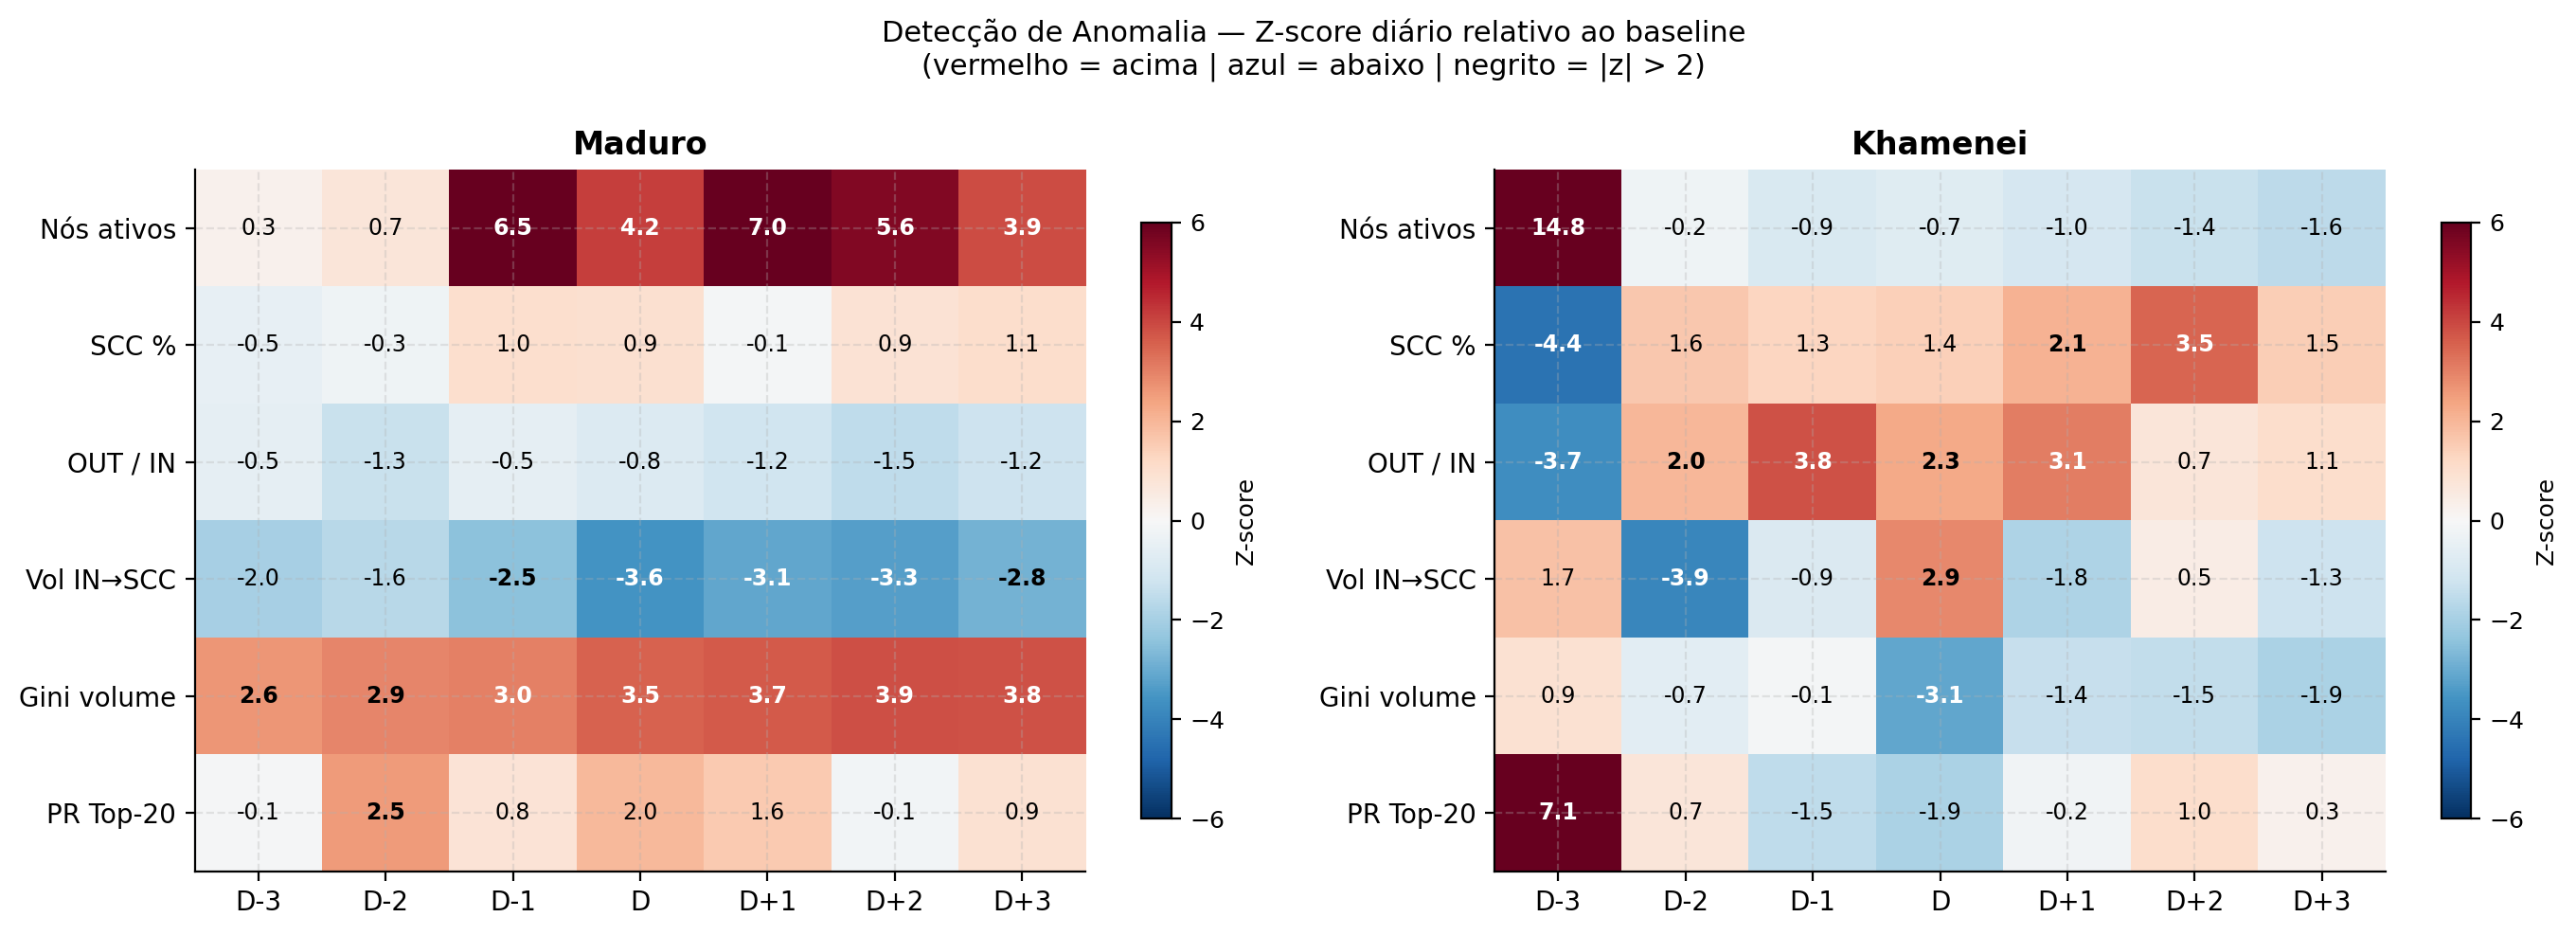
\includegraphics[width=\textwidth]{report_heatmap_zscores.png}
\caption{Heatmap de z-scores diários relativos ao baseline. Valores em negrito indicam $|z| > 2$. O D$-$3 de Khamenei apresenta as anomalias mais extremas do estudo ($z = 14{,}8$ em nós ativos).}
\label{fig:heatmap}
\end{figure}

A evidência on-chain indica que esse pico não está relacionado ao assassinato de Khamenei: o volume de mercado em D$-$3 (283M USD) ficou dentro da faixa normal, sem a explosão que seria esperada de um choque geopolítico, ainda que o número de nós ativos tenha quadruplicado. O descompasso entre volume financeiro normal e atividade on-chain elevada aponta para um evento de mercado de curta duração, e não para acumulação ligada ao evento político. Evidências circunstanciais de fontes secundárias situam nesse dia um \textit{rebound} macro do mercado cripto e o lançamento do par PEPE na Binance, o que seria compatível com a onda de depósitos observada; não confirmamos esses fatos a partir de fontes primárias, e a conclusão de que o pulso é de natureza mercadológica apoia-se na evidência on-chain acima.

\subsubsection{D$-$1 a D$+$3: evento geopolítico}

Após o pulso de D$-$3, o assassinato de Khamenei em D$=$0 teve impacto limitado: o preço caiu 10,9\% ao longo da janela, sem reversão. A rede contraiu para 1.700--2.200 nós por dia, com SCC recuperando para 22,8\% em D$+$2 (consolidação do núcleo). Em D$+$3, o anomaly score caiu para 7,5, dentro da variação normal.

\begin{figure}[H]
\centering
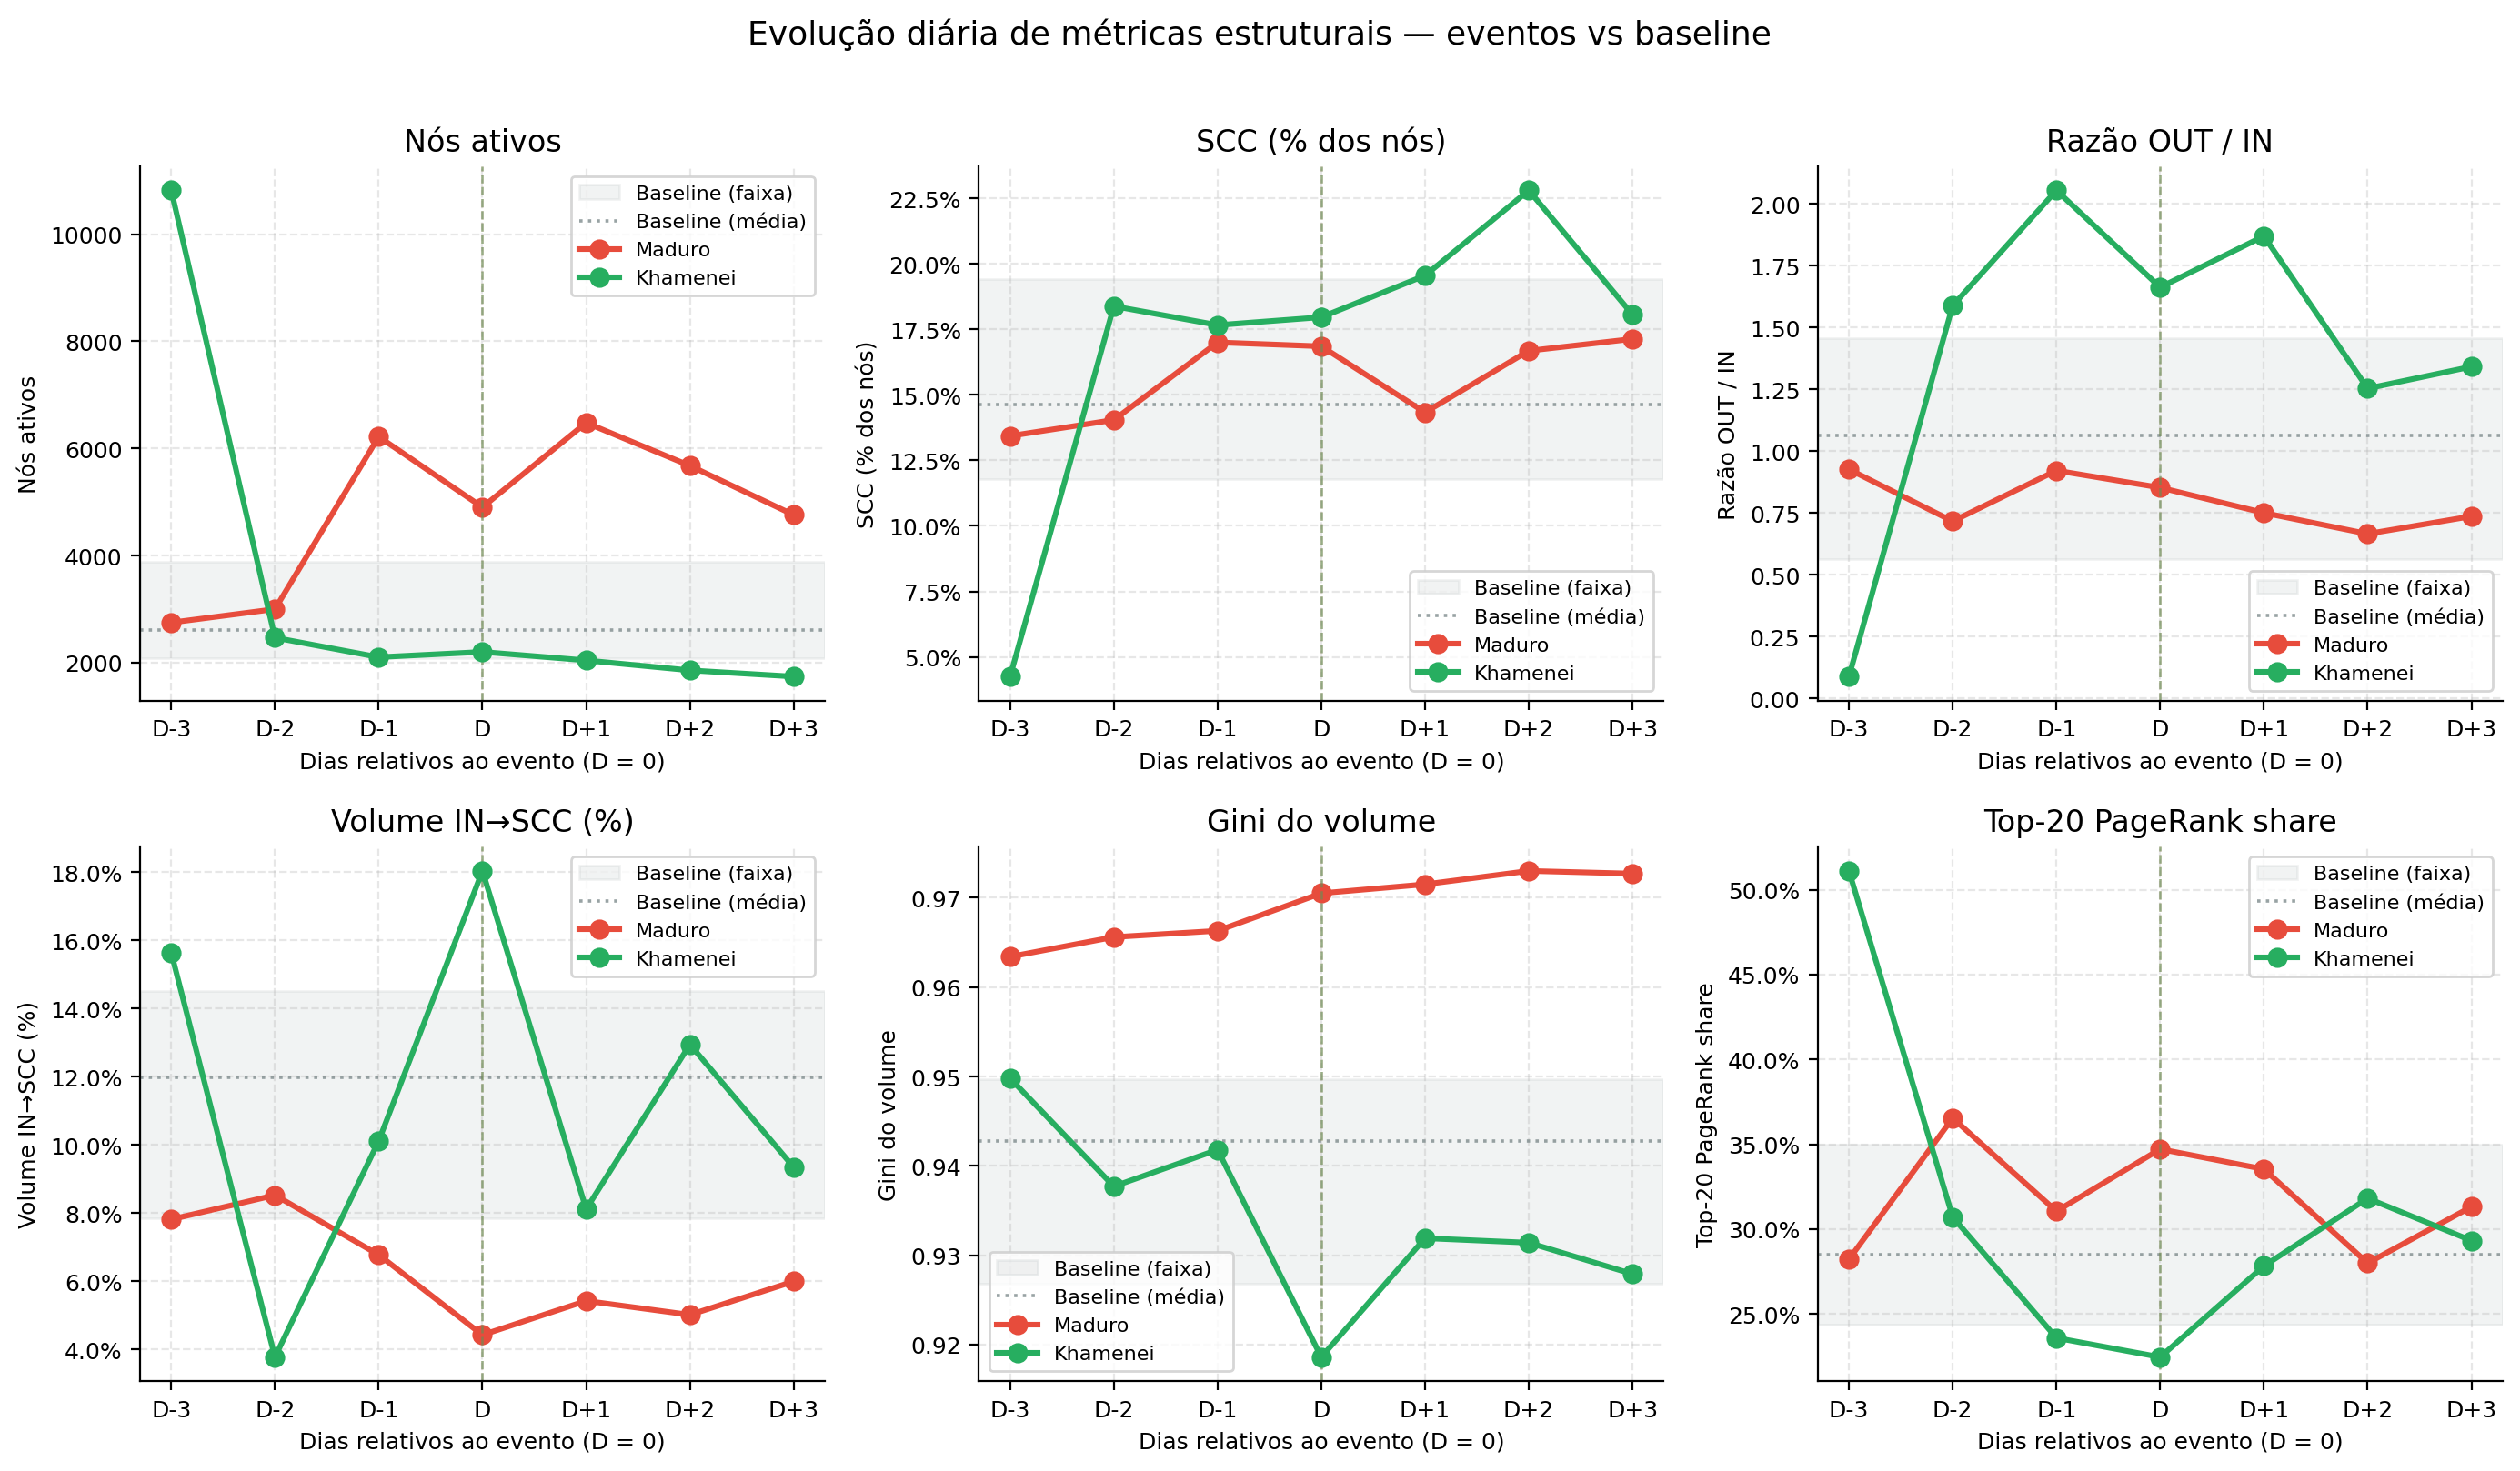
\includegraphics[width=\textwidth]{report_serie_temporal.png}
\caption{Evolução diária de métricas estruturais. A faixa cinza indica a faixa de variação do baseline. O D$-$3 de Khamenei apresenta pico extremo em nós ativos e queda na SCC\%.}
\label{fig:temporal}
\end{figure}

O HITS (não-ponderado, baseado na estrutura de conectividade) no grafo completo Khamenei revelou uma inversão sem precedentes: Gini hub = 0,222 e Gini authority = 1,000. A authority máxima (score = 1,0) é o endereço \texttt{0x28c6c0...}, verificado como a \textbf{hot wallet da Binance}. A inversão indica que milhares de endereços com papel de hub similar (conectando-se às mesmas authorities) coexistem com uma authority ultra-dominante: a Binance, destino de convergência de toda a rede.

Outro endereço relevante no grafo Khamenei é \texttt{0xb334a6...}, verificado como a exchange turca \textbf{BtcTurk}: terceiro no ranking de PageRank (posição 29 no baseline), no $k$-core máximo ($k=8$, percentil 100\%) e com clustering local~=~0 apesar de 132 vizinhos, um perfil de estrela pura compatível com exchange centralizada. A ascensão de rank 29~$\to$~3 é específica ao grafo Khamenei; no grafo Maduro, o mesmo endereço permanece na posição 22, sem salto comparável, o que funciona como controle negativo. Combinando esse dado com o fato de que a Turquia é vizinha e parceira comercial do Irã, e de que o evento Khamenei envolveu o líder supremo iraniano, levantamos a hipótese de que a proeminência da BtcTurk reflete uma resposta desproporcional de investidores com exposição geopolítica regional. Trata-se de uma hipótese, não de um achado confirmado: a verificação definitiva requereria dados de origem geográfica dos depositantes, não disponíveis on-chain.

\subsection{Análise comparativa formal}

\begin{figure}[H]
\centering
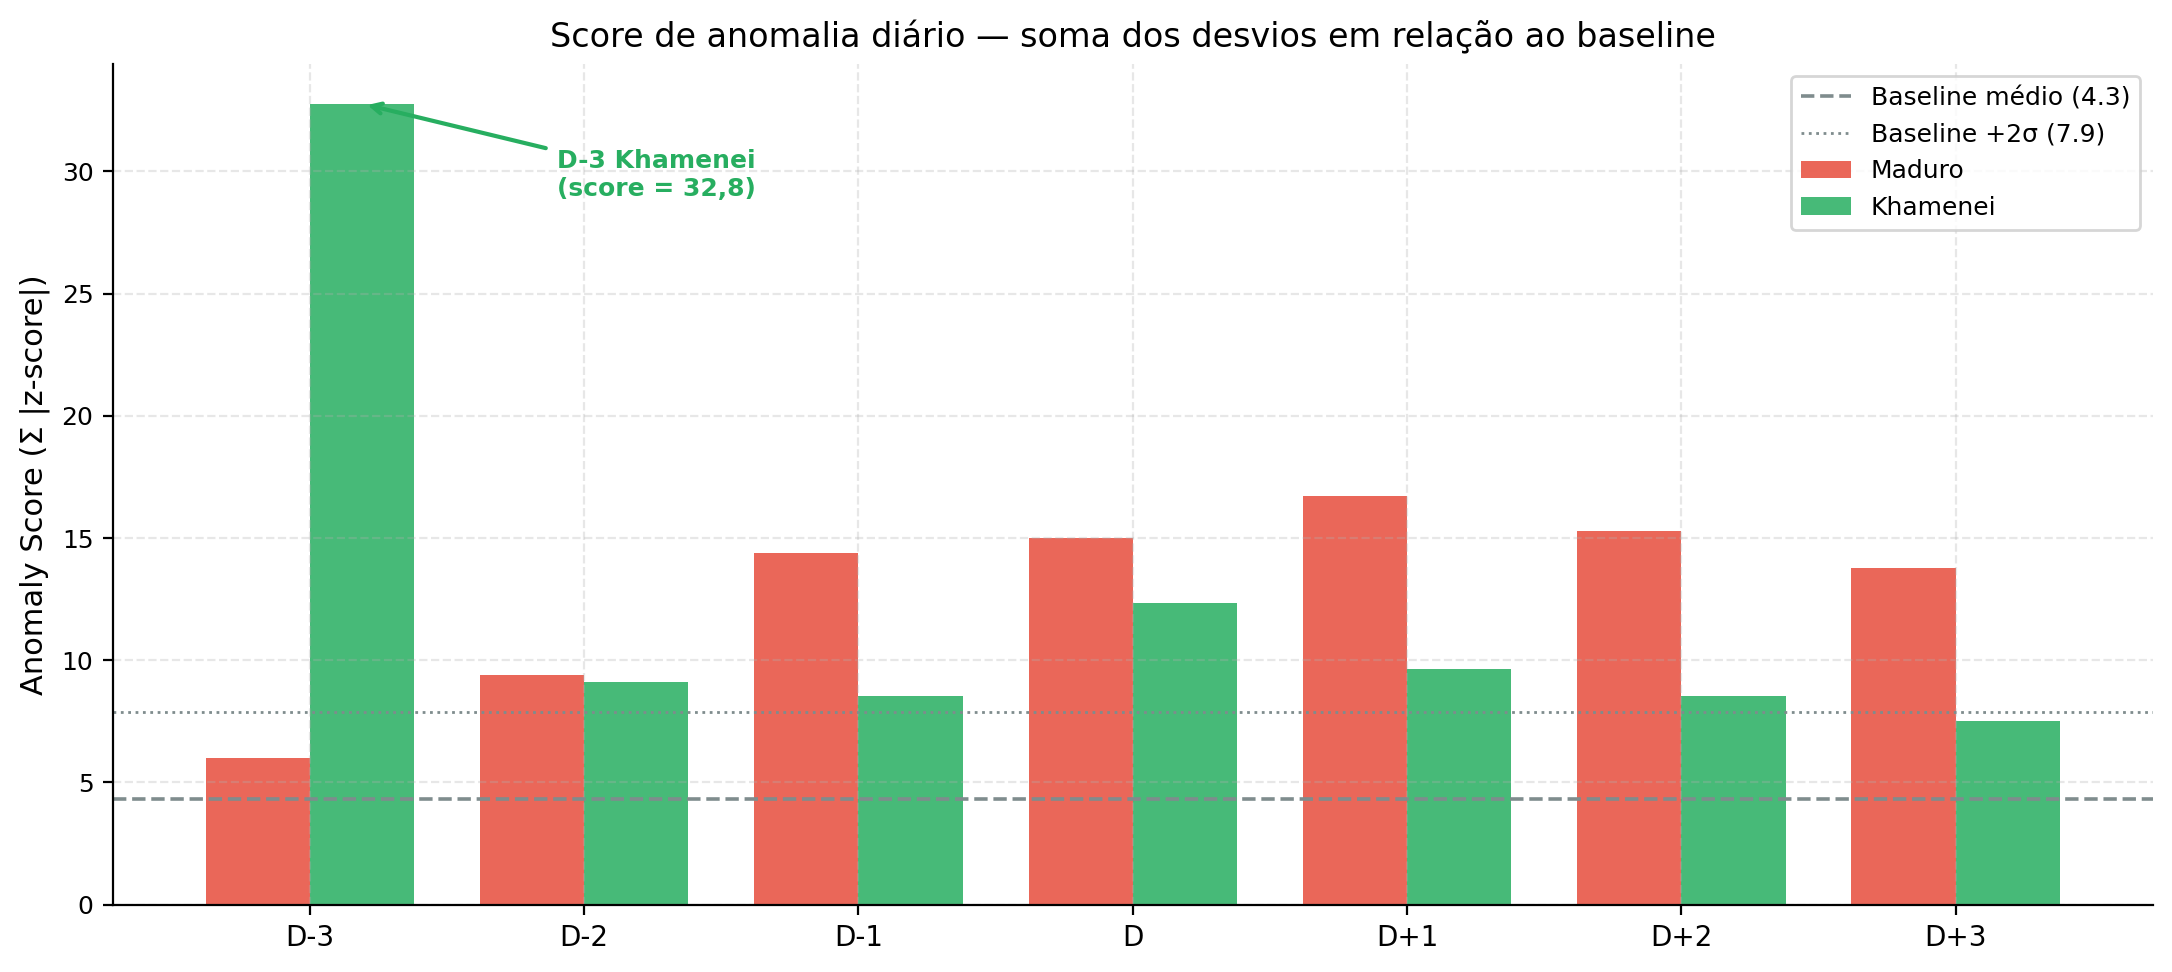
\includegraphics[width=0.85\textwidth]{report_anomaly_score.png}
\caption{Anomaly score diário. O D$-$3 de Khamenei (32,8) é o dia mais anômalo do estudo. Todos os dias do Maduro superam o limiar do baseline.}
\label{fig:anomaly}
\end{figure}

O Maduro apresenta anomalias persistentes: todos os 7 dias têm pelo menos uma métrica com $|z| > 2$, e o anomaly score não retorna ao nível do baseline dentro da janela observada. No Khamenei, o anomaly score cai de 32,8 (D$-$3) para 7,5 em D$+$3, voltando à faixa de variação do baseline. Essa diferença de persistência é coerente com a natureza dos eventos: a incerteza prolongada do caso Maduro está associada a uma perturbação que se mantém por vários dias, ao passo que o pulso de mercado do caso Khamenei se dissipa rapidamente.

A Figura~\ref{fig:hits} ilustra a separação funcional revelada pelo HITS. No baseline e no Khamenei, nenhum endereço aparece simultaneamente no top-20 de hubs e de authorities; no Maduro, apenas 2 endereços ocupam ambas as listas, com perfil de \textit{market-maker} (distribui e acumula). A especialização de papéis é a regra, com essa exceção marginal no grafo mais ativo.

\begin{figure}[H]
\centering
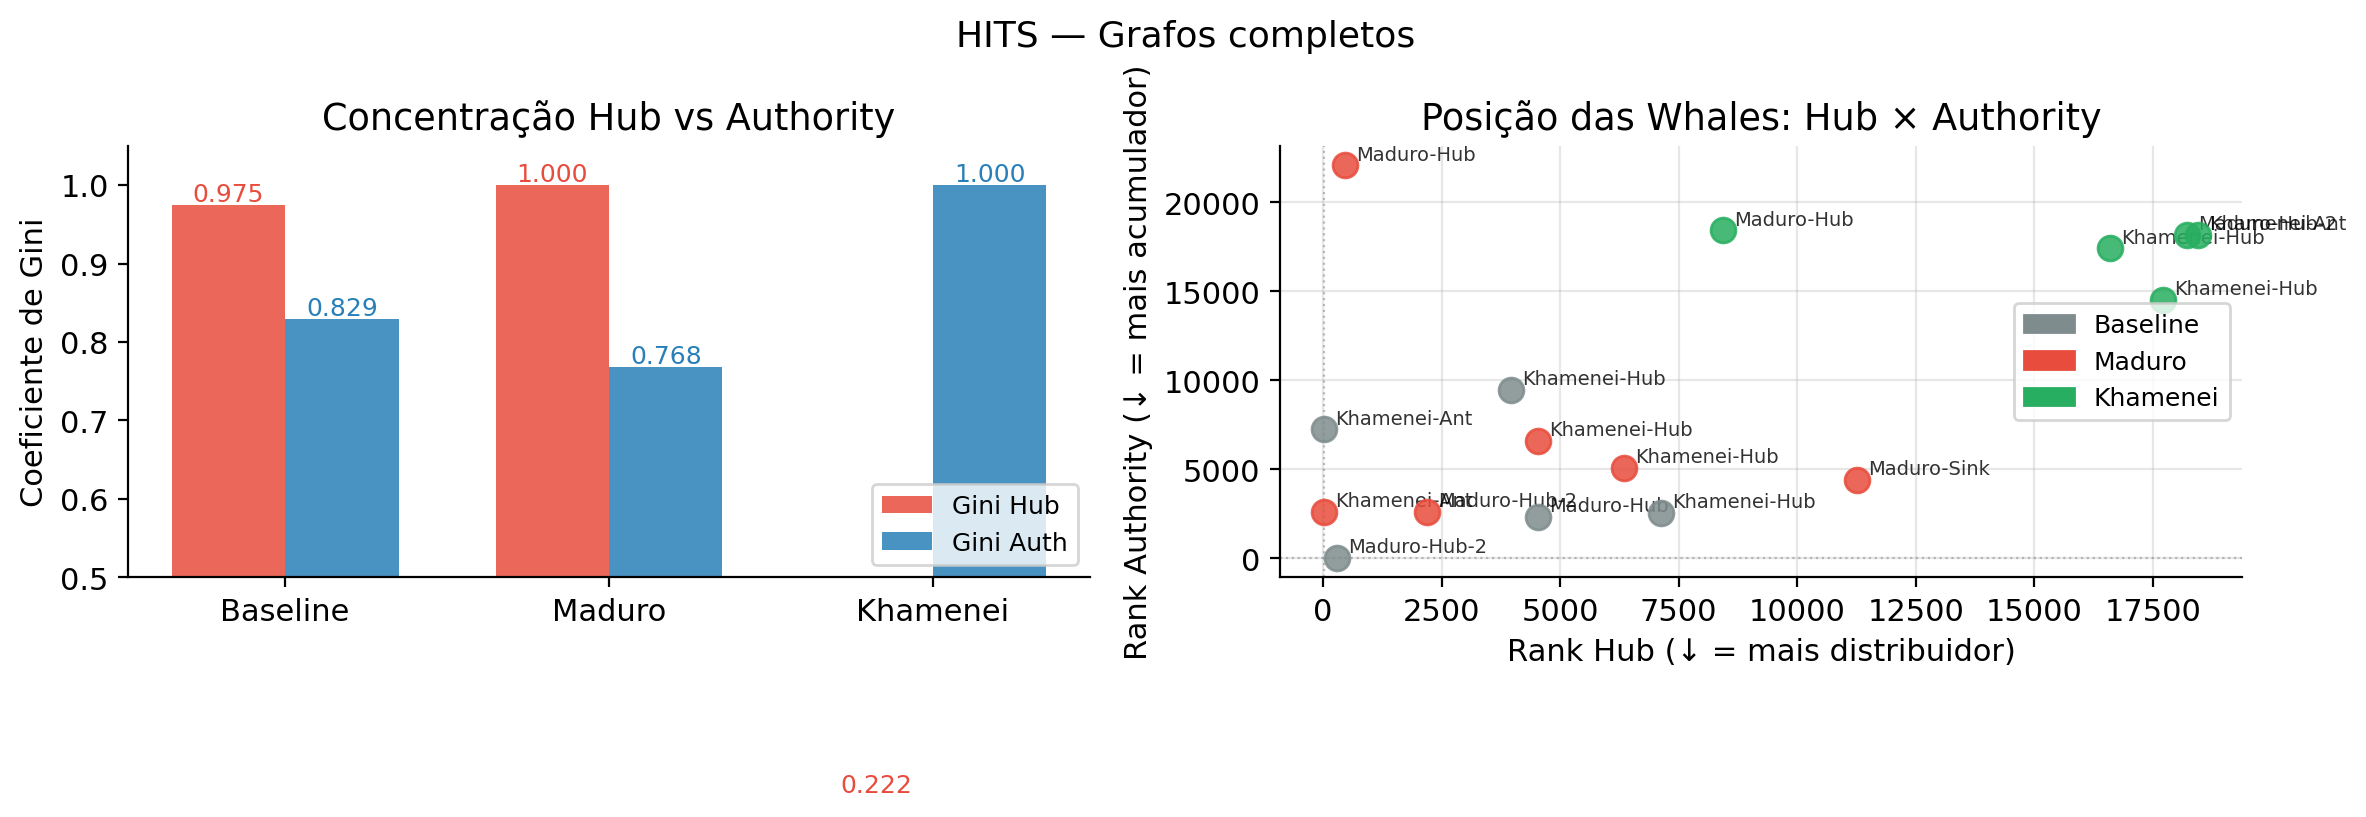
\includegraphics[width=\textwidth]{report_hits_gexf.png}
\caption{HITS: concentração de hubs vs authorities (esquerda) e posição das whales no espaço rank-hub $\times$ rank-authority (direita). A inversão de Gini no Khamenei é visível.}
\label{fig:hits}
\end{figure}

% ============================================================================
\section{Agentes-Chave}
% ============================================================================

A Tabela~\ref{tab:agentes} sintetiza os endereços-chave identificados pela convergência de múltiplos algoritmos. A identificação via Etherscan foi realizada \textit{a posteriori}, após os algoritmos apontarem independentemente para os mesmos endereços:

\begin{table}[H]
\centering
\caption{Endereços-chave verificados via Etherscan.}
\label{tab:agentes}
\small
\begin{tabular}{p{2.5cm}llp{5.5cm}}
\toprule
Endereço & Identificação & Grafo & Papel \\
\midrule
\texttt{0x28c6c0...} & Binance & Khamenei & Authority \#1 (HITS score=1,0). Destino da onda de depósitos. \\
\texttt{0xf97781...} & Binance & Maduro & Sink terminal (4,36T PEPE, zero saídas, $k$=1, comp.\ OUT). \\
\texttt{0x301d9b...} & Phishing\textsuperscript{$\dagger$} & Maduro & Hub \#1 HITS (score=1,0). Criador sinalizado como phishing no Etherscan. \\
\texttt{0xb334a6...} & BtcTurk & Khamenei & PR \#3, $k_{\max}$=8, clustering=0. Exchange turca. \\
\bottomrule
\multicolumn{4}{l}{\footnotesize \textsuperscript{$\dagger$}Padrão estrutural compatível com dust attack ou roteador de liquidez; ver Seção~4.2.}
\end{tabular}
\end{table}

Um achado transversal é que a Binance aparece como destino dominante nos dois eventos, mas em papéis estruturais distintos: sink terminal no Maduro (absorção de capital, $k$-core~=~1, zero saídas) e authority de alta conectividade no Khamenei (HITS~=~1,0, recebendo de milhares de remetentes). O mesmo agente, portanto, é capturado de formas diferentes pelos algoritmos conforme o tipo de fluxo que predomina na janela, o que reforça que a assinatura topológica depende mais do regime de atividade do que da identidade dos endereços envolvidos.

% ============================================================================
\section{Discussão}
% ============================================================================

\subsection{Por que choques diferentes geram redes diferentes?}

A hipótese que emerge dos resultados é que a natureza do choque está associada ao tipo de participante predominante na janela, que por sua vez se reflete na assinatura topológica:

\begin{itemize}[nosep]
\item \textbf{Incerteza prolongada} (Maduro): predomínio de agentes que operam bidirecionalmente ao longo de dias, coincidindo com um núcleo mais denso (SCC$\uparrow$, $k_{\max}\uparrow$, triângulos$\uparrow$).
\item \textbf{Evento de mercado de curta duração} (\textit{rally} macro em D$-$3): predomínio de fluxo unidirecional de varejo em direção a exchange centralizada, associado a uma periferia inflada (IN$\uparrow$, $k$=1$\uparrow$, transitivity$\downarrow$).
\item \textbf{Choque abrupto em mercado de baixa} (assassinato Khamenei): impacto limitado, sem perturbação estrutural destacável sobre a tendência existente.
\end{itemize}

Cabe ressaltar que essa leitura repousa sobre um evento de cada tipo, com uma das janelas contaminada por um sinal de mercado simultâneo. Os padrões descritos devem ser entendidos como hipóteses geradas pelos dados, a serem testadas em um conjunto maior de eventos, e não como relações estabelecidas.

\subsection{Atividade predatória amplificada por volatilidade}

A detecção de um endereço sinalizado como phishing na posição de hub HITS~\#1 durante o período de maior valorização (+73\%) é um achado colateral relevante. Embora a natureza exata do contrato (dust attack vs.\ roteador de liquidez) requeira investigação adicional (Seção~4.2), o padrão estrutural (distribuição massiva para muitas authorities sem reciprocidade) é compatível com atividade predatória amplificada pela euforia de mercado. Isso sugere que a análise de grafos pode contribuir para a segurança on-chain, sinalizando hubs com padrão de distribuição anômalo para inspeção manual.

\subsection{Limitações}

A janela do Khamenei capturou inadvertidamente um evento de mercado (D$-$3), o que exigiu análise temporal para decompor os sinais; essa sobreposição ilustra o desafio de isolar efeitos causais em dados observacionais. O baseline possui apenas 8 observações diárias, tornando os estimadores de média e desvio inerentemente instáveis; z-scores extremos como $z = 14{,}8$ devem ser interpretados qualitativamente (ruptura inequívoca do padrão normal), e não como probabilidades precisas. Dados de preço intraday permitiriam correlação temporal mais fina. A identificação de endereços depende de bases externas (Etherscan) e está sujeita a ambiguidades, como no caso do endereço \texttt{0x301d9b...}, cujo padrão estrutural é compatível tanto com phishing quanto com roteador de liquidez. O estudo mostra correlação topológica, não causalidade. Análises de sensibilidade, como a verificação da estabilidade dos z-scores sob escolha de outro período de baseline, são direções relevantes para trabalho futuro.

% ============================================================================
\section{Conclusão}
% ============================================================================

A análise de oito algoritmos de grafos sobre a rede de transações do token PEPE mostrou que a topologia muda de forma detectável e mensurável diante de eventos externos, e que essas mudanças variam conforme a natureza do evento. Na janela de incerteza prolongada (Maduro), o núcleo bidirecional da rede se adensou; na janela contaminada por um evento de mercado (Khamenei, D$-$3), a periferia unidirecional se inflou; o choque geopolítico isolado em mercado de baixa teve impacto estrutural limitado. Esses padrões emergem de um único evento de cada tipo e devem ser lidos como hipóteses a confirmar.

Vários algoritmos convergiram, de forma independente, sobre os mesmos endereços-chave: a Binance como destino dominante nos dois eventos (em papéis distintos), a BtcTurk como exchange regional com ascensão de ranking específica ao Khamenei, e um endereço sinalizado como phishing na posição de hub mais influente durante a alta de preço. Essa convergência mostra que diferentes métricas de grafo, aplicadas ao mesmo dado on-chain, apontam de forma consistente para os agentes que estruturam a rede em cada regime.

Como trabalho futuro, sugerimos a análise de múltiplos tokens em paralelo, janelas temporais maiores, dados intraday de preço para correlação mais precisa, e desenvolvimento de métodos automatizados de detecção de anomalias topológicas em tempo real.

% ============================================================================
\begin{thebibliography}{9}

\bibitem{barabasi1999}
A.-L.\ Barabási e R.\ Albert, ``Emergence of scaling in random networks,'' \textit{Science}, vol.~286, pp.~509--512, 1999.

\bibitem{page1999}
L.\ Page, S.\ Brin, R.\ Motwani e T.\ Winograd, ``The PageRank citation ranking: Bringing order to the web,'' Stanford InfoLab, Tech.\ Rep., 1999.

\bibitem{kleinberg1999}
J.\ M.\ Kleinberg, ``Authoritative sources in a hyperlinked environment,'' \textit{Journal of the ACM}, vol.~46, no.~5, pp.~604--632, 1999.

\bibitem{broder2000}
A.\ Broder et al., ``Graph structure in the web,'' \textit{Computer Networks}, vol.~33, pp.~309--320, 2000.

\bibitem{batagelj2003}
V.\ Batagelj e M.\ Zaversnik, ``An $O(m)$ algorithm for cores decomposition of networks,'' \textit{arXiv:cs/0310049}, 2003.

\bibitem{alstott2014}
J.\ Alstott, E.\ Bullmore e D.\ Plenz, ``powerlaw: A Python package for analysis of heavy-tailed distributions,'' \textit{PLoS ONE}, vol.~9, no.~1, 2014.

\bibitem{networkx}
A.\ A.\ Hagberg, D.\ A.\ Schult e P.\ J.\ Swart, ``Exploring network structure, dynamics, and function using NetworkX,'' in \textit{Proceedings of SciPy}, 2008.

\end{thebibliography}

\end{document}
